%==============================================================================
% fig_lane_detail.tex  --  detailed SIMTiX warp-pool / lane / FP-unit diagram.
%
% Standalone companion to Fig. 1 of docs/paper/simtix_vlsid.tex, drawn in the
% same visual language (rounded blocks, gray = integer/control, blue = floating
% point, dark gray = storage, white-filled tags on container borders,
% orthogonal edges only).
%
% Panel (a): the four resident warp slots, the round-robin scheduler and its
%            F->X pipeline register, all eight lanes with their per-lane
%            functional units, and the units shared across the lane array.
% Panel (b): the five-stage per-lane FP32/FP16 datapath (simt_fpu), showing the
%            shared fully-pipelined significand multiply and the stage-0 payload
%            delay line that runs in step with it.
%
% Every block corresponds to real RTL:
%   rtl/accel/warp_pool.sv   g_vrf / g_frf / g_fpu / g_imul / g_idot generates,
%                            wstate_e scoreboard, shared fp_divsqrt (M16)
%   rtl/accel/simt_fpu.sv    5-stage pipeline (M15 -> M17 -> B2)
%
% Build:  pdflatex fig_lane_detail
%==============================================================================
\documentclass[border=5mm]{standalone}

\usepackage{amsmath,amssymb}
\usepackage{xcolor}
\usepackage{tikz}
\usetikzlibrary{positioning,fit,backgrounds,arrows.meta,calc}

\begin{document}
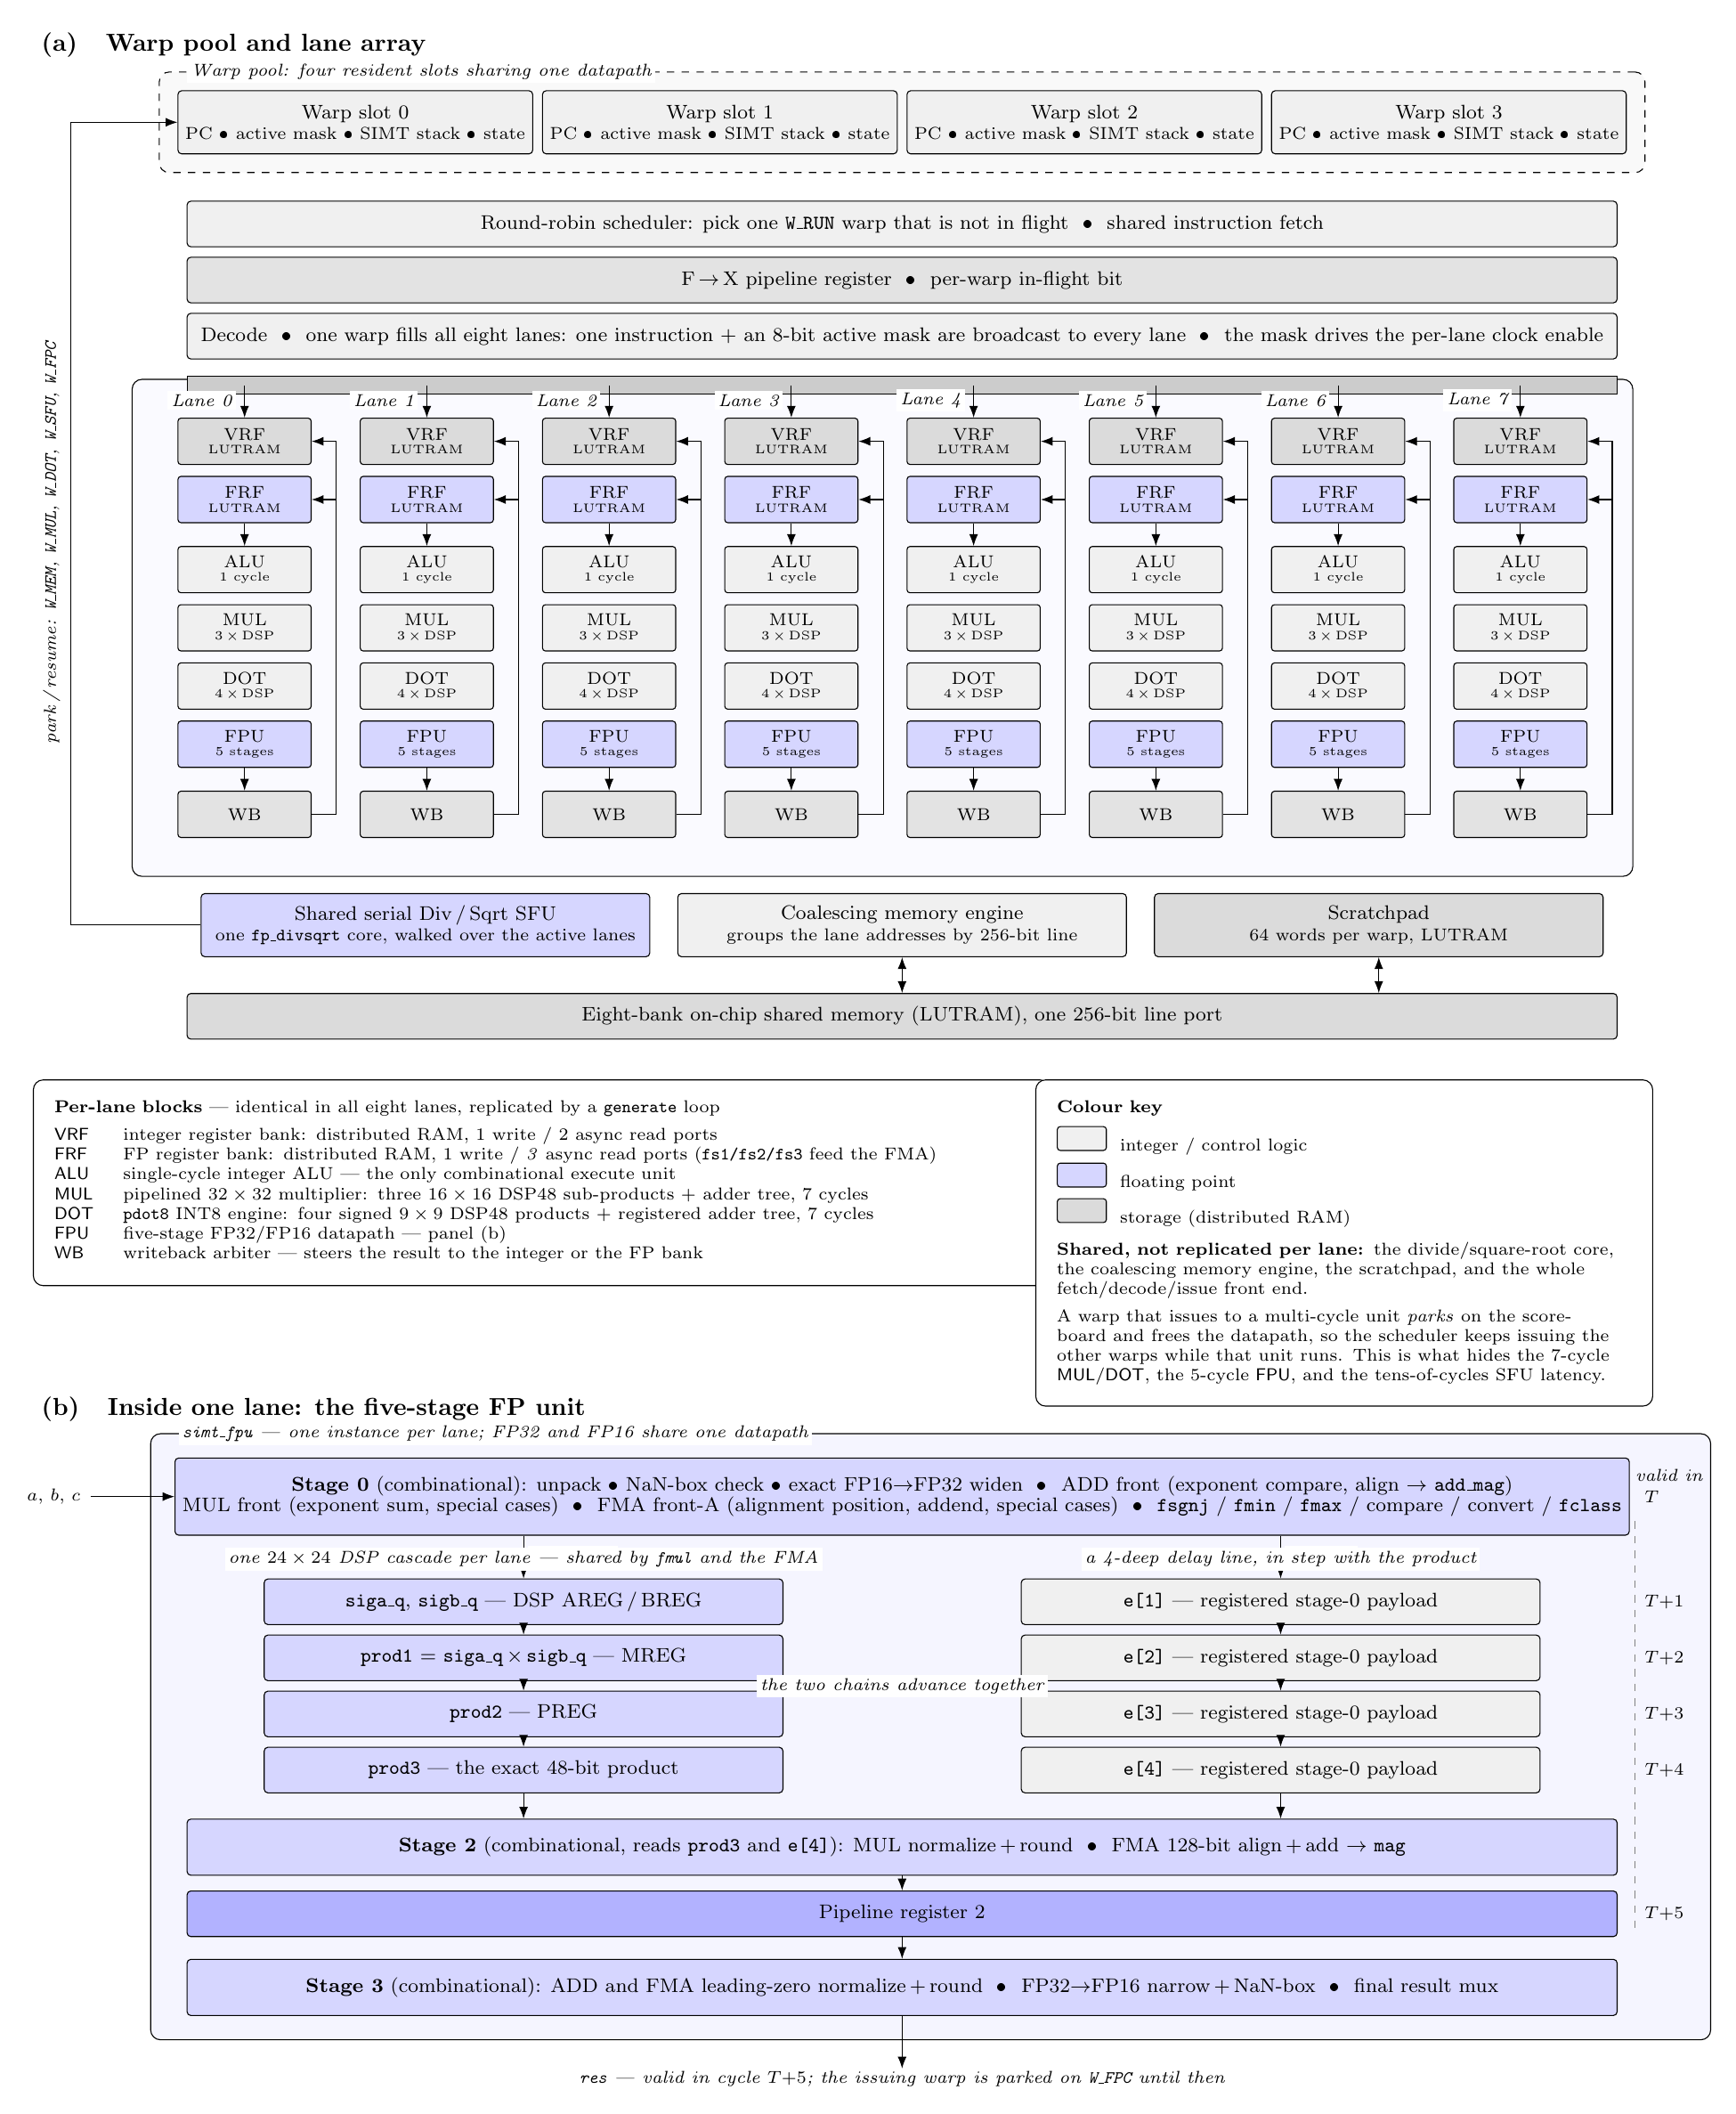
\begin{tikzpicture}[
  font=\footnotesize,
  % ---- block styles (identical palette to Fig. 1 of the paper) ----
  ctl/.style ={draw,rounded corners=1.5pt,align=center,fill=gray!12,
               inner sep=3pt,minimum height=6.5mm},
  fp/.style  ={draw,rounded corners=1.5pt,align=center,fill=blue!16,
               inner sep=3pt,minimum height=6.5mm},
  mem/.style ={draw,rounded corners=1.5pt,align=center,fill=gray!28,
               inner sep=3pt,minimum height=6.5mm},
  unit/.style={draw,rounded corners=1.2pt,align=center,fill=gray!12,
               inner sep=1.5pt,minimum height=6.6mm,minimum width=19mm,
               font=\scriptsize},
  funit/.style={unit,fill=blue!16},
  munit/.style={unit,fill=gray!28},
  lab/.style ={font=\scriptsize\itshape,inner sep=1pt},
  tag/.style ={font=\scriptsize\itshape,fill=white,inner sep=1.5pt},
  panel/.style={font=\bfseries},
  >=Latex
]
\newcommand{\sub}[1]{\\[-2.5pt]{\tiny #1}}

%==============================================================================
% PANEL (a) -- warp pool, scheduler, lane array, shared units
%==============================================================================

% ---- four resident warp slots -----------------------------------------------
\foreach \w/\wx in {0/-7.8, 1/-2.6, 2/2.6, 3/7.8} {
  \node[ctl,minimum width=4.6cm,minimum height=9mm] (warp\w) at (\wx,16.0)
    {Warp slot \w\\[-1pt]
     {\scriptsize PC \textbullet\ active mask \textbullet\ SIMT stack \textbullet\ state}};
}

% ---- scheduler / fetch / decode ---------------------------------------------
\node[ctl,minimum width=20.4cm] (sched) at (0,14.55)
  {Round-robin scheduler: pick one \texttt{W\_RUN} warp that is not in flight
   \ \textbullet\ \ shared instruction fetch};
\node[ctl,minimum width=20.4cm,fill=gray!22] (fx) at (0,13.75)
  {F\,$\rightarrow$\,X pipeline register \ \textbullet\ \ per-warp in-flight bit};
\node[ctl,minimum width=20.4cm] (dec) at (0,12.95)
  {Decode \ \textbullet\ \ one warp fills all eight lanes: one instruction + an
   8-bit active mask are broadcast to every lane
   \ \textbullet\ \ the mask drives the per-lane clock enable};

% ---- issue broadcast bus ----------------------------------------------------
\node[draw,fill=gray!40,minimum width=20.4cm,minimum height=2.6mm,
      inner sep=0pt] (bus) at (0,12.25) {};

% ---- the eight lanes --------------------------------------------------------
% lane k is centred at x = -9.1 + 2.6k ; blocks sit left of an internal
% writeback rail so the rail never crosses a block.
\foreach \l in {0,...,7} {
  \pgfmathsetmacro{\cx}{-9.1 + 2.6*\l}
  \pgfmathsetmacro{\bx}{\cx - 0.28}     % block centre
  \pgfmathsetmacro{\rx}{\cx + 1.03}     % writeback rail

  \node[munit]  (vrf\l)  at (\bx,11.45) {VRF\sub{LUTRAM}};
  \node[funit]  (frf\l)  at (\bx,10.62) {FRF\sub{LUTRAM}};
  \node[unit]   (alu\l)  at (\bx, 9.62) {ALU\sub{1 cycle}};
  \node[unit]   (mul\l)  at (\bx, 8.79) {MUL\sub{3\,$\times$\,DSP}};
  \node[unit]   (dot\l)  at (\bx, 7.96) {DOT\sub{4\,$\times$\,DSP}};
  \node[funit]  (fpu\l)  at (\bx, 7.13) {FPU\sub{5 stages}};
  \node[unit,fill=gray!22] (wb\l) at (\bx, 6.13) {WB};

  % operand read into the execute units, result into the writeback arbiter
  \draw[->] (frf\l.south) -- (alu\l.north);
  \draw[->] (fpu\l.south) -- (wb\l.north);
  % writeback rail: WB back up into the two register banks
  \draw[->] (wb\l.east) -- (\rx,6.13) -- (\rx,11.45) -- (vrf\l.east);
  \draw[->] (\rx,10.62) -- (frf\l.east);

  % lane container + tag
  \begin{scope}[on background layer]
    \node[fit=(vrf\l)(frf\l)(alu\l)(mul\l)(dot\l)(fpu\l)(wb\l),
          draw,rounded corners,inner xsep=3.4mm,inner ysep=2.4mm,
          fill=blue!3] (lane\l) {};
  \end{scope}
  \node[tag,anchor=west] at ($(lane\l.north west)+(2mm,0)$) {Lane \l};

  % issue fan-out
  \draw[->] (\bx,12.25) -- (vrf\l.north);
}

% ---- units shared by the whole lane array -----------------------------------
\node[fp,minimum width=6.4cm,minimum height=9mm]  (sfu)  at (-6.8,4.55)
  {Shared serial Div\,/\,Sqrt SFU\\[-1pt]
   {\scriptsize one \texttt{fp\_divsqrt} core, walked over the active lanes}};
\node[ctl,minimum width=6.4cm,minimum height=9mm] (memeng) at (0,4.55)
  {Coalescing memory engine\\[-1pt]
   {\scriptsize groups the lane addresses by 256-bit line}};
\node[mem,minimum width=6.4cm,minimum height=9mm] (spad) at (6.8,4.55)
  {Scratchpad\\[-1pt]
   {\scriptsize 64 words per warp, LUTRAM}};

\node[mem,minimum width=20.4cm] (smem) at (0,3.25)
  {Eight-bank on-chip shared memory (LUTRAM), one 256-bit line port};

\draw[<->] (memeng.south) -- (memeng.south|-smem.north);
\draw[<->] (spad.south)   -- (spad.south|-smem.north);

% ---- park / resume scoreboard feedback --------------------------------------
\draw[->] (sfu.west) -- ++(-1.85,0) |- (warp0.west);
\node[tag,rotate=90,anchor=south] at (-11.95,10.0)
  {park\,/\,resume: \texttt{W\_MEM}, \texttt{W\_MUL}, \texttt{W\_DOT},
   \texttt{W\_SFU}, \texttt{W\_FPC}};

% ---- containers -------------------------------------------------------------
\begin{scope}[on background layer]
  \node[fit=(warp0)(warp3),draw,dashed,rounded corners,inner sep=2.6mm,
        fill=gray!5] (pool) {};
  \node[fit=(lane0)(lane7),draw,rounded corners,inner sep=3.0mm,
        fill=blue!2] (array) {};
\end{scope}
\node[tag,anchor=west] at ($(pool.north west)+(4mm,0)$)
  {Warp pool: four resident slots sharing one datapath};
% (the lane array needs no title tag: every lane carries its own, and the decode
%  box above already states that one warp fills all eight lanes)

% ---- legend -----------------------------------------------------------------
\node[draw,rounded corners,align=left,inner sep=3mm,fill=white,font=\scriptsize,
      anchor=north west,text width=13.9cm] (keyL) at (-12.4,2.35) {%
  \textbf{Per-lane blocks} --- identical in all eight lanes, replicated by a
  \texttt{generate} loop\\[3pt]
  \begin{tabular}{@{}ll@{}}
    \textsf{VRF} & integer register bank: distributed RAM, 1 write / 2 async read ports\\
    \textsf{FRF} & FP register bank: distributed RAM, 1 write / \emph{3} async read ports
                   (\texttt{fs1/fs2/fs3} feed the FMA)\\
    \textsf{ALU} & single-cycle integer ALU --- the only combinational execute unit\\
    \textsf{MUL} & pipelined $32\times32$ multiplier: three $16\times16$ DSP48
                   sub-products + adder tree, 7 cycles\\
    \textsf{DOT} & \texttt{pdot8} INT8 engine: four signed $9\times9$ DSP48 products
                   + registered adder tree, 7 cycles\\
    \textsf{FPU} & five-stage FP32/FP16 datapath --- panel (b)\\
    \textsf{WB}  & writeback arbiter --- steers the result to the integer or the FP bank\\
  \end{tabular}};

\node[draw,rounded corners,align=left,inner sep=3mm,fill=white,font=\scriptsize,
      anchor=north west,text width=8.2cm] (keyR) at (1.9,2.35) {%
  \textbf{Colour key}\\[3pt]
  \tikz\node[unit,minimum width=7mm,minimum height=3.4mm]{};~~integer / control logic\\[2pt]
  \tikz\node[funit,minimum width=7mm,minimum height=3.4mm]{};~~floating point\\[2pt]
  \tikz\node[munit,minimum width=7mm,minimum height=3.4mm]{};~~storage (distributed RAM)\\[5pt]
  \textbf{Shared, not replicated per lane:} the divide/square-root core, the
  coalescing memory engine, the scratchpad, and the whole fetch/decode/issue
  front end.\\[3pt]
  A warp that issues to a multi-cycle unit \emph{parks} on the scoreboard and
  frees the datapath, so the scheduler keeps issuing the other warps while that
  unit runs. This is what hides the 7-cycle \textsf{MUL}/\textsf{DOT}, the
  5-cycle \textsf{FPU}, and the tens-of-cycles SFU latency.};

\node[panel,anchor=north west] at (-12.4,17.4) {(a)\quad Warp pool and lane array};

%==============================================================================
% PANEL (b) -- the five-stage per-lane FP datapath (simt_fpu)
%==============================================================================
\def\py{-3.6}   % vertical origin of panel (b)

\node[fp,minimum width=20.4cm,minimum height=11mm] (s0) at (0,\py+0.0)
  {\textbf{Stage 0} (combinational): unpack \textbullet\ NaN-box check
   \textbullet\ exact FP16$\rightarrow$FP32 widen
   \ \textbullet\ \ ADD front (exponent compare, align $\rightarrow$ \texttt{add\_mag})\\[-1pt]
   MUL front (exponent sum, special cases) \ \textbullet\ \ FMA front-A (alignment
   position, addend, special cases)
   \ \textbullet\ \ \texttt{fsgnj} / \texttt{fmin} / \texttt{fmax} / compare /
   convert / \texttt{fclass}};

\node[lab,anchor=east] at ($(s0.west)+(-13mm,0)$) {$a,\,b,\,c$};
\draw[->] ($(s0.west)+(-12mm,0)$) -- (s0.west);

% --- left chain: the shared fully-pipelined significand multiply -------------
\node[fp,minimum width=7.4cm] (dsp0) at (-5.4,\py-1.50)
  {\texttt{siga\_q}, \texttt{sigb\_q} --- DSP AREG\,/\,BREG};
\node[fp,minimum width=7.4cm] (dsp1) at (-5.4,\py-2.30)
  {\texttt{prod1} $=$ \texttt{siga\_q}\,$\times$\,\texttt{sigb\_q} --- MREG};
\node[fp,minimum width=7.4cm] (dsp2) at (-5.4,\py-3.10)
  {\texttt{prod2} --- PREG};
\node[fp,minimum width=7.4cm] (dsp3) at (-5.4,\py-3.90)
  {\texttt{prod3} --- the exact 48-bit product};

\draw[->] (s0.south-|dsp0) -- (dsp0.north)
          node[tag,midway,right,xshift=1.5pt] {\texttt{siga},\,\texttt{sigb}};
\draw[->] (dsp0) -- (dsp1);
\draw[->] (dsp1) -- (dsp2);
\draw[->] (dsp2) -- (dsp3);

\node[tag,anchor=south] at (-5.4,\py-1.06)
  {one $24\times24$ DSP cascade per lane --- shared by \texttt{fmul} and the FMA};

% --- right chain: the stage-0 payload delay line -----------------------------
\foreach \i/\dy in {1/-1.50, 2/-2.30, 3/-3.10, 4/-3.90} {
  \node[ctl,minimum width=7.4cm] (e\i) at (5.4,\py+\dy)
    {\texttt{e[\i]} --- registered stage-0 payload};
}
\draw[->] (s0.south-|e1) -- (e1.north)
          node[tag,midway,right,xshift=1.5pt] {payload};
\draw[->] (e1) -- (e2);
\draw[->] (e2) -- (e3);
\draw[->] (e3) -- (e4);

\node[tag,anchor=south] at (5.4,\py-1.06)
  {a 4-deep delay line, in step with the product};

\node[tag] at (0,\py-2.70) {the two chains advance together};

% --- stage 2 ------------------------------------------------------------------
\node[fp,minimum width=20.4cm,minimum height=8mm] (s2) at (0,\py-5.00)
  {\textbf{Stage 2} (combinational, reads \texttt{prod3} and \texttt{e[4]}):
   MUL normalize\,+\,round \ \textbullet\ \ FMA 128-bit align\,+\,add
   $\rightarrow$ \texttt{mag}};
\draw[->] (dsp3.south) -- (dsp3.south|-s2.north);
\draw[->] (e4.south)   -- (e4.south|-s2.north);

\node[fp,minimum width=20.4cm,fill=blue!30] (r2) at (0,\py-5.95)
  {Pipeline register 2};
\draw[->] (s2) -- (r2);

% --- cycle axis: one label per register boundary, shared by both chains -------
\foreach \c/\cy in {0/0.00, 1/-1.50, 2/-2.30, 3/-3.10, 4/-3.90, 5/-5.95} {
  \node[lab,anchor=west] (t\c) at (10.55,\py+\cy)
    {\ifnum\c=0 $T$\else $T{+}\c$\fi};
}
\draw[gray,dashed,thin] (10.45,\py-0.35) -- (10.45,\py-6.25);
\node[lab,anchor=west] (thead) at (10.42,\py+0.30) {valid in};

\node[fp,minimum width=20.4cm,minimum height=8mm] (s3) at (0,\py-7.00)
  {\textbf{Stage 3} (combinational): ADD and FMA leading-zero normalize\,+\,round
   \ \textbullet\ \ FP32$\rightarrow$FP16 narrow\,+\,NaN-box
   \ \textbullet\ \ final result mux};
\draw[->] (r2) -- (s3);

\draw[->] (s3.south) -- ++(0,-0.75)
  node[lab,anchor=north,align=center]
  {\texttt{res} --- valid in cycle $T{+}5$; the issuing warp is parked on
   \texttt{W\_FPC} until then};

\begin{scope}[on background layer]
  \node[fit=(s0)(dsp3)(e4)(s2)(r2)(s3)(t0)(t5),draw,rounded corners,inner sep=3.4mm,
        fill=blue!4] (fpubox) {};
\end{scope}
\node[tag,anchor=west] at ($(fpubox.north west)+(4mm,0)$)
  {\texttt{simt\_fpu} --- one instance per lane; FP32 and FP16 share one datapath};

\node[panel,anchor=north west] at (-12.4,\py+1.55)
  {(b)\quad Inside one lane: the five-stage FP unit};

\end{tikzpicture}
\end{document}
